% Source: graduate-coursework/Research/Intro_to_Agents/handouts/Part8_Advanced_Topics.tex

\documentclass[border=4pt]{standalone}
\usepackage[T1]{fontenc}
\usepackage{graphicx}
\usepackage{lmodern}
\usepackage{tikz}
\usepackage{xcolor}
\usetikzlibrary{shapes.geometric, arrows.meta, positioning, calc, fit, backgrounds, matrix, decorations.pathreplacing}

\definecolor{UofSCGarnet}{HTML}{73000a}
\definecolor{UofSCBlack}{HTML}{000000}
\definecolor{UofSCWhite}{HTML}{ffffff}
\definecolor{UofSCRose}{HTML}{CC2E40}
\definecolor{UofSCAtlantic}{HTML}{466A9F}
\definecolor{UofSCCongaree}{HTML}{1F414D}
\definecolor{UofSCHorseshoe}{HTML}{65780B}
\definecolor{UofSCGrass}{HTML}{CED318}
\definecolor{UofSCHoneycomb}{HTML}{A49137}
\definecolor{UofSC90Black}{HTML}{363636}
\definecolor{UofSC70Black}{HTML}{5C5C5C}
\definecolor{UofSC50Black}{HTML}{A2A2A2}
\definecolor{UofSCWarmGrey}{HTML}{676156}
\definecolor{UofSCSandstorm}{HTML}{FFF2E3}
\definecolor{UofSCDarkGarnet}{HTML}{570008}
\definecolor{UofSCAzalea}{HTML}{844247}

\tikzset{
    % Sharp corners for all nodes
    every node/.style={font=\small},
    % Process box style
    process/.style={
        rectangle,
        draw=UofSCBlack,
        fill=UofSCWhite,
        minimum width=2.5cm,
        minimum height=0.8cm,
        align=center,
        font=\footnotesize
    },
    % Decision box style
    decision/.style={
        diamond,
        draw=UofSCBlack,
        fill=UofSCSandstorm,
        minimum width=2cm,
        minimum height=1cm,
        align=center,
        font=\footnotesize,
        aspect=2
    },
    % Start/End style
    startstop/.style={
        rectangle,
        draw=UofSCGarnet,
        fill=UofSCGarnet,
        text=UofSCWhite,
        minimum width=2cm,
        minimum height=0.7cm,
        align=center,
        font=\footnotesize\bfseries
    },
    % Arrow style
    arrow/.style={
        ->,
        >=Stealth,
        thick,
        color=UofSCBlack
    },
    % Failure node
    failure/.style={
        rectangle,
        draw=UofSCRose,
        fill=UofSCRose!20,
        minimum width=2cm,
        minimum height=0.7cm,
        align=center,
        font=\footnotesize
    },
    % Success node
    success/.style={
        rectangle,
        draw=UofSCHorseshoe,
        fill=UofSCHorseshoe!20,
        minimum width=2cm,
        minimum height=0.7cm,
        align=center,
        font=\footnotesize
    },
    % Highlight box
    highlight/.style={
        rectangle,
        draw=UofSCGarnet,
        fill=UofSCGarnet!10,
        line width=1.5pt,
        minimum width=2.5cm,
        minimum height=0.8cm,
        align=center,
        font=\footnotesize
    },
    % Security threat style
    threat/.style={
        rectangle,
        draw=UofSCRose,
        fill=UofSCRose!15,
        minimum width=2.2cm,
        minimum height=0.7cm,
        align=center,
        font=\footnotesize
    },
    % Agent node
    agent/.style={
        rectangle,
        draw=UofSCAtlantic,
        fill=UofSCAtlantic!15,
        minimum width=2.2cm,
        minimum height=0.8cm,
        align=center,
        font=\footnotesize
    },
    % Human node
    human/.style={
        rectangle,
        draw=UofSCCongaree,
        fill=UofSCCongaree!15,
        minimum width=2.2cm,
        minimum height=0.8cm,
        align=center,
        font=\footnotesize
    },
    % Cost node
    cost/.style={
        rectangle,
        draw=UofSCHoneycomb,
        fill=UofSCHoneycomb!20,
        minimum width=2cm,
        minimum height=0.7cm,
        align=center,
        font=\footnotesize
    },
    % Test node
    test/.style={
        rectangle,
        draw=UofSCAtlantic,
        fill=UofSCAtlantic!10,
        minimum width=2cm,
        minimum height=0.7cm,
        align=center,
        font=\footnotesize
    },
    % Pipeline stage
    pipeline/.style={
        rectangle,
        draw=UofSCCongaree,
        fill=UofSCCongaree!10,
        minimum width=2.5cm,
        minimum height=0.8cm,
        align=center,
        font=\footnotesize
    },
    % Timeline event
    timeline/.style={
        rectangle,
        draw=UofSCGarnet,
        fill=UofSCWhite,
        minimum width=1.8cm,
        minimum height=0.6cm,
        align=center,
        font=\tiny
    }
}

\begin{document}
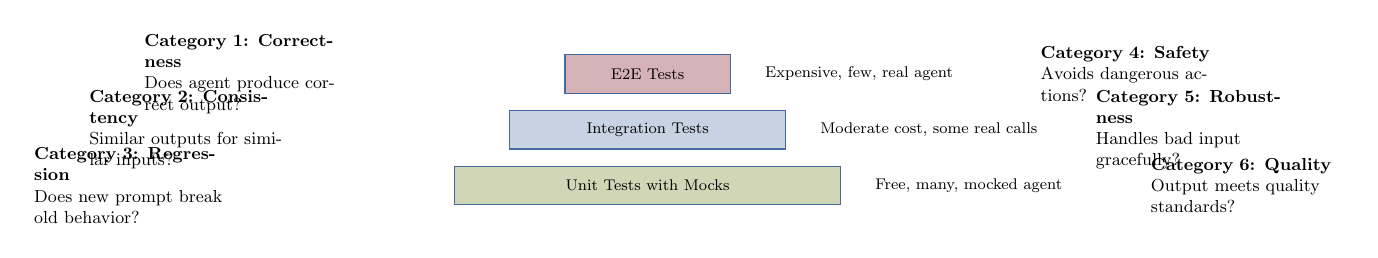
\begin{tikzpicture}[node distance=0.3cm and 0.5cm, scale=0.7, transform shape]
        % Testing Pyramid
        \node (e2e) [test, minimum width=3cm, fill=UofSCGarnet!30] {E2E Tests};
        \node (int) [test, below=of e2e, minimum width=5cm, fill=UofSCAtlantic!30] {Integration Tests};
        \node (unit) [test, below=of int, minimum width=7cm, fill=UofSCHorseshoe!30] {Unit Tests with Mocks};

        % Labels
        \node [right=0.5cm of e2e, font=\footnotesize, text width=4cm] {Expensive, few, real agent};
        \node [right=0.5cm of int, font=\footnotesize, text width=4cm] {Moderate cost, some real calls};
        \node [right=0.5cm of unit, font=\footnotesize, text width=4cm] {Free, many, mocked agent};

        % Categories on left
        \node [left=4cm of e2e, text width=3.5cm, font=\small] {
            \textbf{Category 1: Correctness}\\
            Does agent produce correct output?
        };
        \node [left=4cm of int, text width=3.5cm, font=\small] {
            \textbf{Category 2: Consistency}\\
            Similar outputs for similar inputs?
        };
        \node [left=4cm of unit, text width=3.5cm, font=\small] {
            \textbf{Category 3: Regression}\\
            Does new prompt break old behavior?
        };

        % Right side categories
        \node [right=5.5cm of e2e, text width=3.5cm, font=\small] {
            \textbf{Category 4: Safety}\\
            Avoids dangerous actions?
        };
        \node [right=5.5cm of int, text width=3.5cm, font=\small] {
            \textbf{Category 5: Robustness}\\
            Handles bad input gracefully?
        };
        \node [right=5.5cm of unit, text width=3.5cm, font=\small] {
            \textbf{Category 6: Quality}\\
            Output meets quality standards?
        };
    \end{tikzpicture}
\end{document}
